O principal resultado deste trabalho foi fazer o \emph{Boinc} funcionar com rotinas em \emph{R}, tanto
nos ambientes \emph{Linux} como no ambiente \emph{Windows} % colocar marca registrada

\subsection{Implementação}

\subsubsection{Sistema Linux}

Para o ambiente \emph{Linux}, o processo foi relativamente simples: dado um arquivo com rotinas
do \emph{R} a serem executadas, é somente necessário alterar a permissão do arquivo para executável 
(via \verb#chmod +x arquivo.R#) e adicionar a seguinte linha no início do arquivo:

\begin{verbatim}
#!/usr/bin/Rscript
\end{verbatim}

Isso faz um sistema \emph{Linux} chamar o interpretador \emph{Rscript} para interpretar o arquivo  
e assim fazer a interpretação do arquivo. Esta solução permite não só que rotinas em \emph{R} sejam
executadas, mas sim qualquer script que tenha seu interpretador descrito na primeira linha.

A esta solução, demos o nome de \emph{Truque do Shebang}, pelos caracteres \verb'#!' serem chamados
popularmente de \emph{shebang}. Esta implementação foi relativamente simples: o BOINC possuía um tutorial
para executarmos programas compilados na grade e só o truque do shebang foi necessário.

Porém, para termos a mesma solução em ambos os sistemas, utilizamos a solução para 
Windows no sistema Linux. 

\subsubsection{Sistema Windows} %Marca registrada

Como o sistema Windows não permite utilizar script utilizando o \emph{shebang}, foi necessário 
utilizar um programa compilado escrito na linguagem C, que chamamos de \emph{Runner}, 
que usando a função \verb#system#, chama o interpretador com o arquivo.R como parâmetro. 

Esta solução permite inclusive que usemos scripts diferentes de R a cada vez que criamos um 
\emph{workunit}, assim como adicionar arquivos extra que por ventura fossem necessários para
o processamento. Esta maneira também funciona no \emph{Linux}, só que o \emph{Runner} precisa
ser compilado para o \emph{Linux} com o caminho para o interpretador correto. O programa também não faz
uma verificação para perceber se o \emph{R} está instalado, dando um resultado de conclusão positiva
no banco, mas sem arquivos de saída. 

A utilização do \emph{Runner} foi necessária devido ao \emph{Wrapper} não perceber corretamente
que o interpretador foi executado sem erros e, mesmo em execuções sem erros, o \emph{wrapper} 
recebia um valor de retorno do interpretador diferente de zero, o que ele percebia como um erro
e marcava o \emph{workunit} como inválido. Um diagrama exemplificando esse funcionamento pode ser visto 
na figura \ref{diagrama-boinc-wrapper-windows}. Para a execução ficar multiplataforma, foi necessário 
fazer uma pequena alteração no \emph{wrapper} na versão para \emph{Linux} modificando o nome do
arquivo XML do wrapper, já que em ambos os sistemas é necessária a utilização de um arquivo XML próprio.


A implementação no Windows foi bastante difícil: existem muitos pequenos detalhes que acabam
atrapalhando um pouco. Um dos exemplos foi especificar o caminho do executável: para o Windows acessar
um diretório específico devemos ``truncar'' os nomes de diretórios maiores que $8$ caracteres, sendo 
assim apontamos o caminho, trocando o oitavo e nono caractere do diretório por \verb#~1# 
e desprezando os seguintes. 
Alguns outros problemas foram relacionados à falta de mensagens de erro do BOINC mais amigáveis e
à falta de verificação das entradas: um \verb#XML# mal formatado causou um erro  no processamento
do workunit, quando isso deveria ser acusado na submissão do workunit. Outro problema foi um \emph{Bug}
nas configurações de compilação do \emph{wrapper} no Microsoft Visual Studio Express % Verificar 
que fazia referência a bibliotecas desnecessárias e inexistentes para a compilação do \emph{wrapper}
e isso só foi resolvido pelos desenvolvedores do \emph{BOINC} algumas semanas depois. 


\begin{figure}[!h]
  \centering
  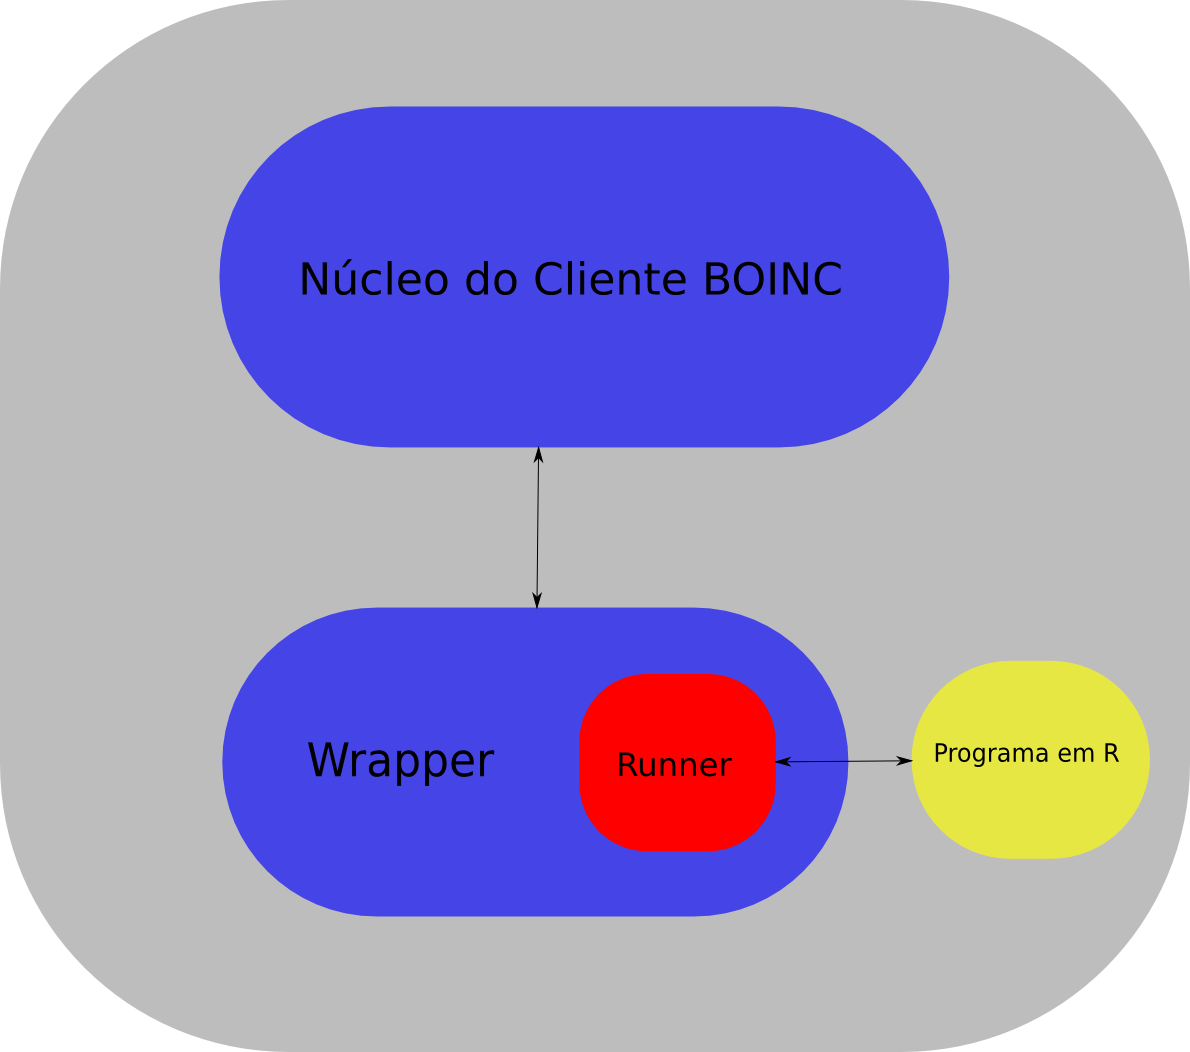
\includegraphics[scale=0.3]{boinc-diagram-runner.png}
  \caption{Diagrama do funcionamento do \emph{BOINC} com o \emph{Runner} e \emph{Wrapper}}
  \label{diagrama-boinc-wrapper-windows}
\end{figure}
 

\subsection{Discussão}



\subsubsection{Vantagens} 

As principais vantagens no uso do \emph{Boinc} para o processamento em grade são:

\begin{itemize}
  \item \textbf{Facilidade de se adicionar novos nós} - A instalação do BOINC em ambos os sistemas Linux e Windows é simples
e fácil de ser feita e nenhuma ação no servidor é necessária a cada instalação de nós. Além disso, é muito simples fazer
a replicação de configurações, tanto para o processamento, quanto para a conexão com o servidor para os computadores;
  \item \textbf{Processamento multiplataforma} - Para a grade funcionar na plataforma só são necessárias duas coisas: 
que o BOINC e o \emph{R} estejam disponível para a plataforma. As plataformas mais comuns 
(Linux $32$ e $64$ bits e Microsoft Windows) têm ambos os projetos disponíveis;
  \item \textbf{Código aberto} - A utilização de dois softwares com código aberto facilita bastante: a 
busca de bugs se torna possível, a gratuidade dos softwares e a grande quantidade de documentação, muitas vezes produzidas por
pessoas que não necessariamente são da equipe de desenvolvimento do \emph{BOINC}. A mentalidade de ajuda mútua, existente nas
listas de discussão e no canal de IRC do projeto também é de grande ajuda; 
  \item \textbf{Execução invisível ao usuário} - Com o \emph{BOINC} configurado para isso, um usuário comum da rede nem ao menos 
percebe a existência de um processamento em grade. É possível configurar o \emph{BOINC} para só começar a execução com o computador ocioso
após um número arbitrário de minutos. Também é possível configurar para o processamento só acontecer em determinadas 
faixas de horários e dias da semana. Outra configuração interessante é a determinação do máximo de memória 
\emph{RAM} e de espaço em disco para a execução, assim como a frequência com que ele usará a rede. 
  \item \textbf{Solução funciona para qualquer linguagem de script} - De maneira análoga, é possível executar qualquer programa escrito em 
linguagem interpretada com o BOINC utilizando esta mesma solução. Como comentado antes, só é necessário que exista uma versão do interpretador
para as plataformas necessárias (o que é comum para as linguagens mais utilizadas como \emph{PERL}, \emph{Python} e 
\emph{Ruby} e as plataformas mais comuns). 

\end{itemize}

\subsubsection{Desvantagens}

As principais desvantagens são:

\begin{itemize}
  \item \textbf{Necessidade de se ter o \emph{R} instalado} - O \emph{R} não é uma linguagem ins\-ta\-la\-da por padrão
nas distribuições Linux mais populares, nem no \emph{Windows}. Então, a adição de um nó só pode ser feita se o \emph{R}
for também instalado. 
  \item \textbf{Falta de checkpoints} - Utilizando um aplicativo feito com a \emph{API} do \emph{BOINC} é possível se ter
\emph{Checkpoints}, que são uma maneira de uma aplicação feita com o \emph{BOINC} reiniciar o processamento
não do início, mas sim de um determinado ponto. Utilizando o \emph{Wrapper} e o \emph{R}, perdemos esse recurso. A computação
de rotinas longas se torna mais difícil e pouco recomendada, já que a cada interrupção o processamento é reiniciado. 
  \item \textbf{Falta de ``compromisso'' fixo dos clientes} - Diferentemente da rede citada no artigo \cite{Dias}
não há a figura de um computador \emph{Manager} que gerencia as máquinas, atualizando a qualquer momento, mas sim um servidor 
que apenas envia e recebe as tarefas e a iniciativa de computação fica com os computadores da grade. 

\end{itemize}

\subsection{Instalação da rede}

A instalação para o sistema Linux foi concluída no laboratório CEC do IME-USP. No momento possuímos $69$ máquinas com o sistema 
Linux funcionando plenamente e 2 máquinas com algum problema na instalação dos pacotes 
necessários para a computação.  

No momento está sendo feito a instalação no sistema Windows que contará com $16$ máquinas que possuem um dual-boot
com máquinas com o sistema Linux já presentes na grade. Esta instalação se mostrou um pouco mais complexa, de\-vi\-do a 
configurações que devem ser feitas no momento da instalação (e cuja necessidade é pouco clara na documentação).

Somente três alterações foram feitas na configuração dos clientes: 


\begin{itemize}
   \item Execução das tarefas apenas quando o computador estiver ocioso por $10min$. Por padrão, o \textit{Boinc} é 
executado sempre, inclusive quando um usuário esteja usando. Como nossa intenção é executar no tempo ocioso da rede, 
escolhemos essa configuração. 
   \item Conexão com o servidor sempre que possível. Como normalmente a distância de um cliente para um servidor é longa,
a conexão com o servidor é feito apenas após um período determinado de tempo (por padrão $0.10 dia$). Reduzimos 
esse valor para zero, tornando a transmissão de resultados sempre que possível devido ao baixo volume de dados transmitidos. 
   \item \emph{Buffer} de tarefas adicionais ajustada para zero. Por padrão, o cliente do \textit{Boinc} assume o processamento de várias
tarefas de uma vez, e devolvendo o resultado de todas estas ao mesmo tempo. Porém para distribuir melhor as
tarefas nos nós e devido a comunicação com o servidor ser frequente (como especificado no item anterior)
reduzimos o acúmulo de tarefas com o servidor para zero.
\end{itemize} 


\subsection{Testes}

Para testar a grade foi criado um script na linguagem \emph{R} que apenas fazia contas sem significado 
por, aproximadamente, $4min20s$ ``dedicados'' (isto é, executados diretamente em um dos computadores da grade). Foram criados 
$150$ \textit{workunits} para serem distribuídos entre as máquinas  processadas. Como
configurado no servidor, foi utilizada uma redundância que enviava, 
para cada \textit{workunit}, duas tarefas a serem processadas.

Devido a utilização do CEC no mês de janeiro e início de feveiro para cursos de verão (no qual um deles utilizou o sistema em uma das salas Windows), somente duas máquinas fizeram o processamento das $300$ tarefas. O tempo médio 
de processamento das tarefas foi de $9min2.167s$, com um desvio padrão de $14.486s$. Um histograma desta execução pode 
ser encontrado na figura \ref{hist_tarefas}. Um dos computadores (que chamarei de $1$) teve um desempenho pouco superior ao outro tendo uma
média de $8min50.130s$ (e um desvio padrão de $6.543s$) contra uma média de $9min16.404s$ (com um desvio padrão de $5.544s$) do outro computador (chamado de $2$). Os histogramas do tempo de execução nos computadores podem ser encontrados na figura \ref{hist_comp1} e \ref{hist_comp2} para os computadores $1$ e $2$, respectivamente. O computador $1$ processou $154$ tarefas, contra $146$ do computador $2$. Todas 
execuções foram feitas com sucesso e todos os resultados gerados estão presentes no diretório de upload dos resultados. 

\begin{figure}[!ht]
	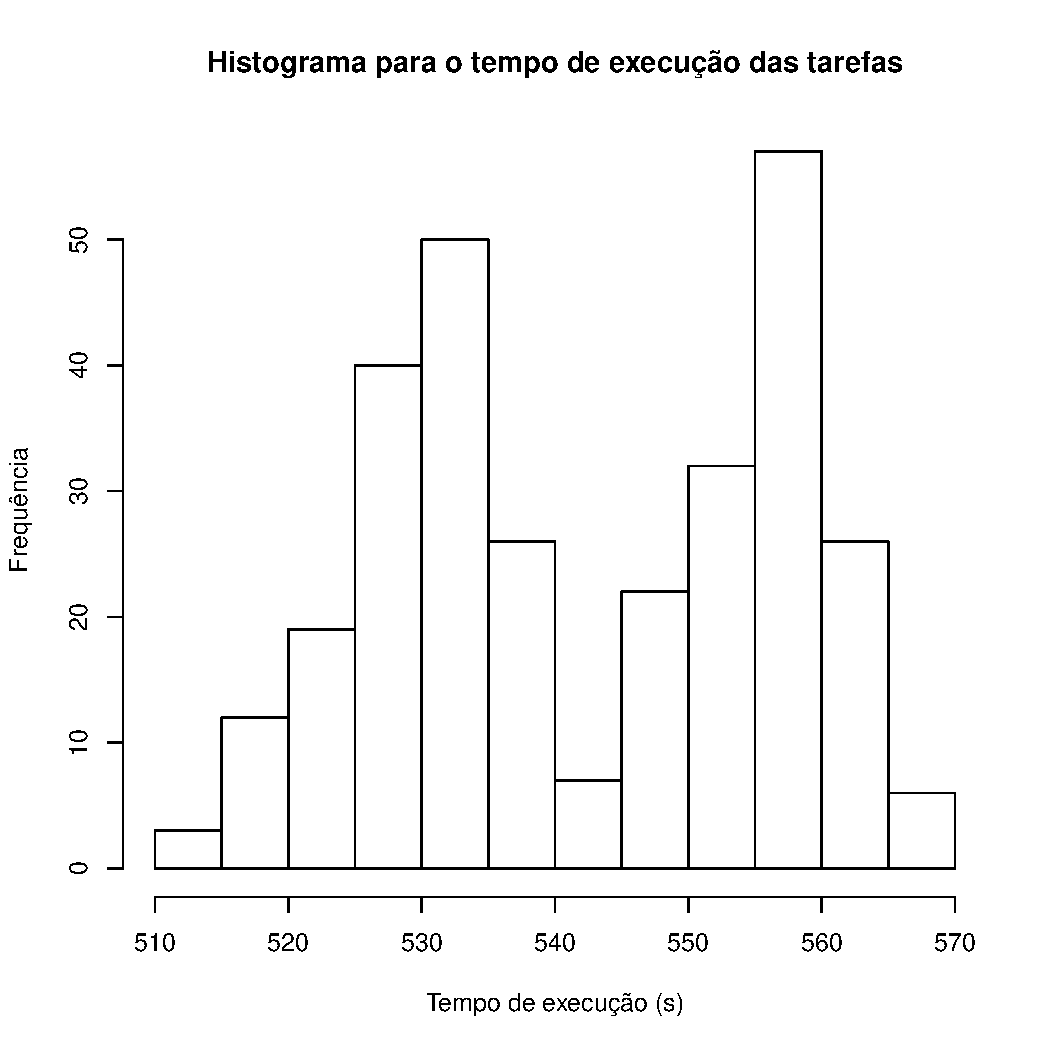
\includegraphics[scale=0.8]{hist_geral.pdf}

	\caption{Histograma dos tempos de execução das tarefas}
	\label{hist_tarefas}
\end{figure}


\begin{figure}[!ht]
	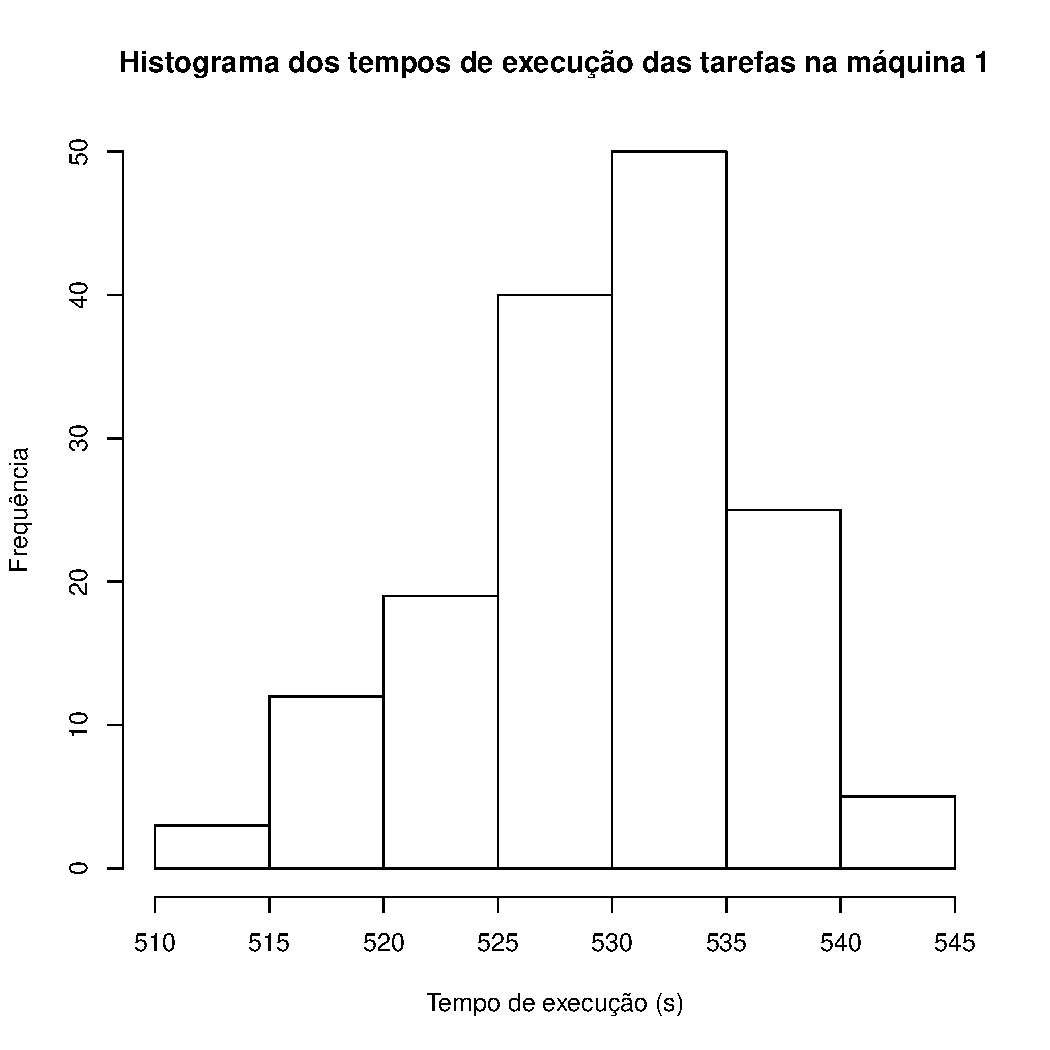
\includegraphics[scale=0.8]{hist1.pdf}

	\caption{Histograma dos tempos de execução das tarefas no computador $1$}
	\label{hist_comp1}
\end{figure}


\begin{figure}[!ht]
	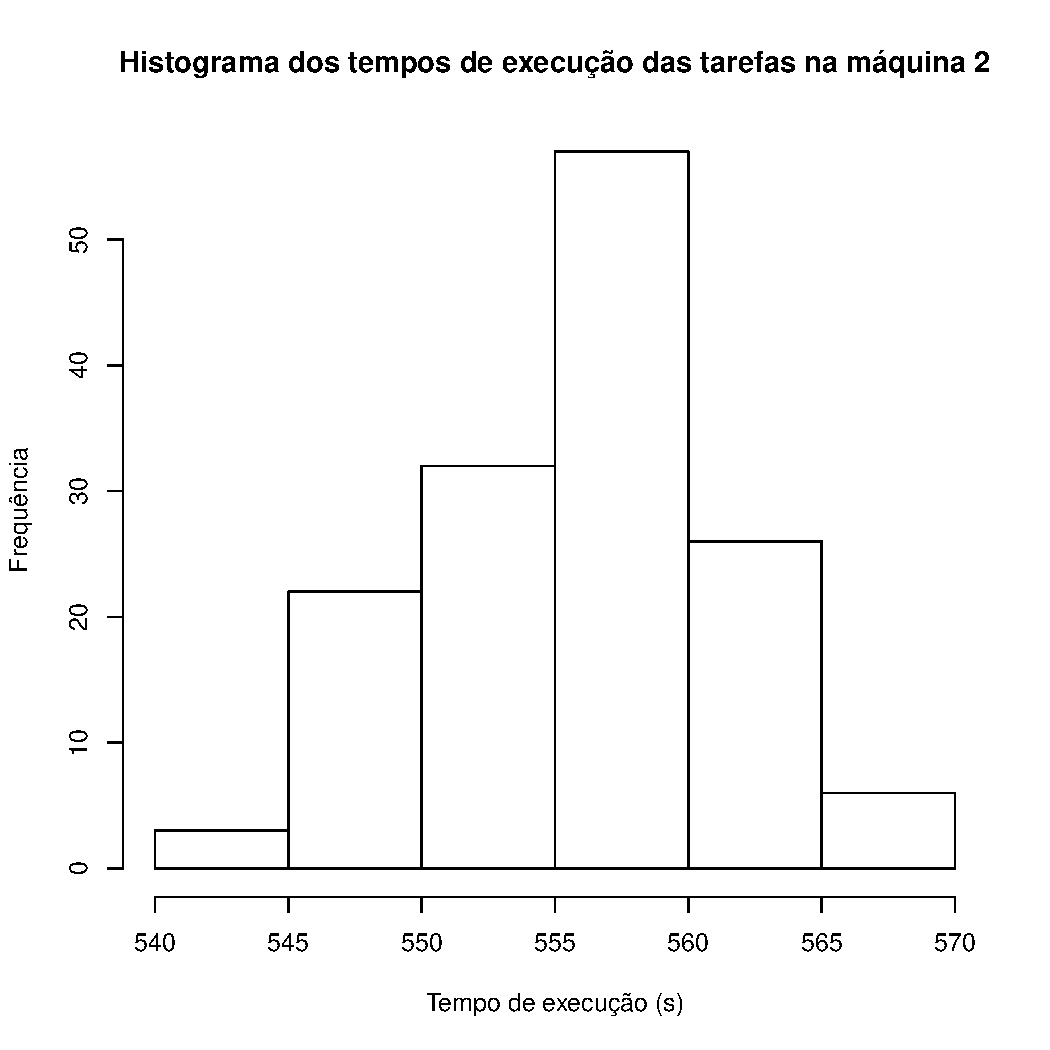
\includegraphics[scale=0.8]{hist2.pdf}

	\caption{Histograma dos tempos de execução das tarefas no computador $2$}
	\label{hist_comp2}	
\end{figure}



O tempo total de processamento das tarefas foi de $14h31min41s$. Caso as tarefas fossem processadas
em série, em um computador e de maneira direta (sem o \emph{BOINC})
o tempo de execução seria de, aproximadamente, $21h40min$ o que nos dá um \emph{speed-up} 
próximo de $1.5$.








